\chapter{Modele rozmyte Takagiego--Sugeno}
\section{Zmienna reguł i dyskretne modele lokalne}
Zmienną przesłanek jest poziom $h_2$, od którego zależy przekrój drugiego zbiornika $B_2(h_2)=3C_2h_2^2$ oraz reakcja układu na niemierzalne zakłócenie $F_D$. Zakres $h_2\in[\num{4.500},\ \num{26.538}]\ \mathrm{cm}$ odpowiada zmianom dopływu $\uvar$ od 50 do 150~$\jednprzep$ ($\pm50\%$) przy $F_{D,0}=20\ \jednprzep$. Podzielono go równomiernie na 2, 3, 4 i 5~węzłów z trójkątnymi funkcjami przynależności (z ramionami na brzegach), sumującymi się do jedności.

W każdym węźle $h_{2,i}$ wyznaczono punkt równowagi $q_i=\alpha_2\sqrt{h_{2,i}}$, $h_{1,i}=(q_i/\alpha_1)^2$ oraz linearyzację obiektu:
\begin{align}
\dot h &= A_i(h-h_i)+B\bigl(\uvar(t-\tau)+F_D(t)-q_i\bigr),\\
A_i&=\begin{bmatrix}-k_{1,i}/A_1&0\\k_{1,i}/B_{2,i}&-k_{2,i}/B_{2,i}\end{bmatrix},\quad
B=\begin{bmatrix}1/A_1\\0\end{bmatrix},\\
k_{1,i}&=\frac{\alpha_1}{2\sqrt{h_{1,i}}},\quad
k_{2,i}=\frac{\alpha_2}{2\sqrt{h_{2,i}}},\quad B_{2,i}=3C_2h_{2,i}^2.
\end{align}
Modele lokalne zdyskretyzowano metodą ZOH (\texttt{c2d}, $T_s=20\ \mathrm{s}$) do równań różnicowych (materiały wykładowe \emph{Modele rozmyte}, s.~133--134, wzory (4.38) i (4.41)):
\begin{align}
 y^i(k+1)&=b_{1,i}\,y(k)+b_{2,i}\,y(k-1)+c_{1,i}\,q(k)+c_{2,i}\,q(k-1)+a_{0,i}^q,\\
 y(k+1)&=\sum_{i=1}^r\widetilde w_i\bigl(y(k)\bigr)\,y^i(k+1),\qquad
 \widetilde w_i(h_2)=\frac{\mu_i(h_2)}{\sum_{\ell=1}^r\mu_\ell(h_2)},
\end{align}
gdzie $q(k)=\uvar(k-10)+F_D(k)$ oraz $a_{0,i}^q=(1-b_{1,i}-b_{2,i})h_{2,i}-(c_{1,i}+c_{2,i})q_i$. W modelach używanych przez regulatory zakłada się nominalne $F_D=F_{D,0}=20\ \jednprzep$, co daje $y^i(k+1)=b_{1,i}y(k)+b_{2,i}y(k-1)+c_{1,i}u(k-10)+c_{2,i}u(k-11)+a_{0,i}$ dla $a_{0,i}=(1-b_{1,i}-b_{2,i})h_{2,i}-(c_{1,i}+c_{2,i})(q_i-F_{D,0})$. Próby rozpoczynano w nominalnym punkcie pracy $h_{2,0}\approx\num{13.223}\ \mathrm{cm}$.

\begin{figure}[H]
\centering
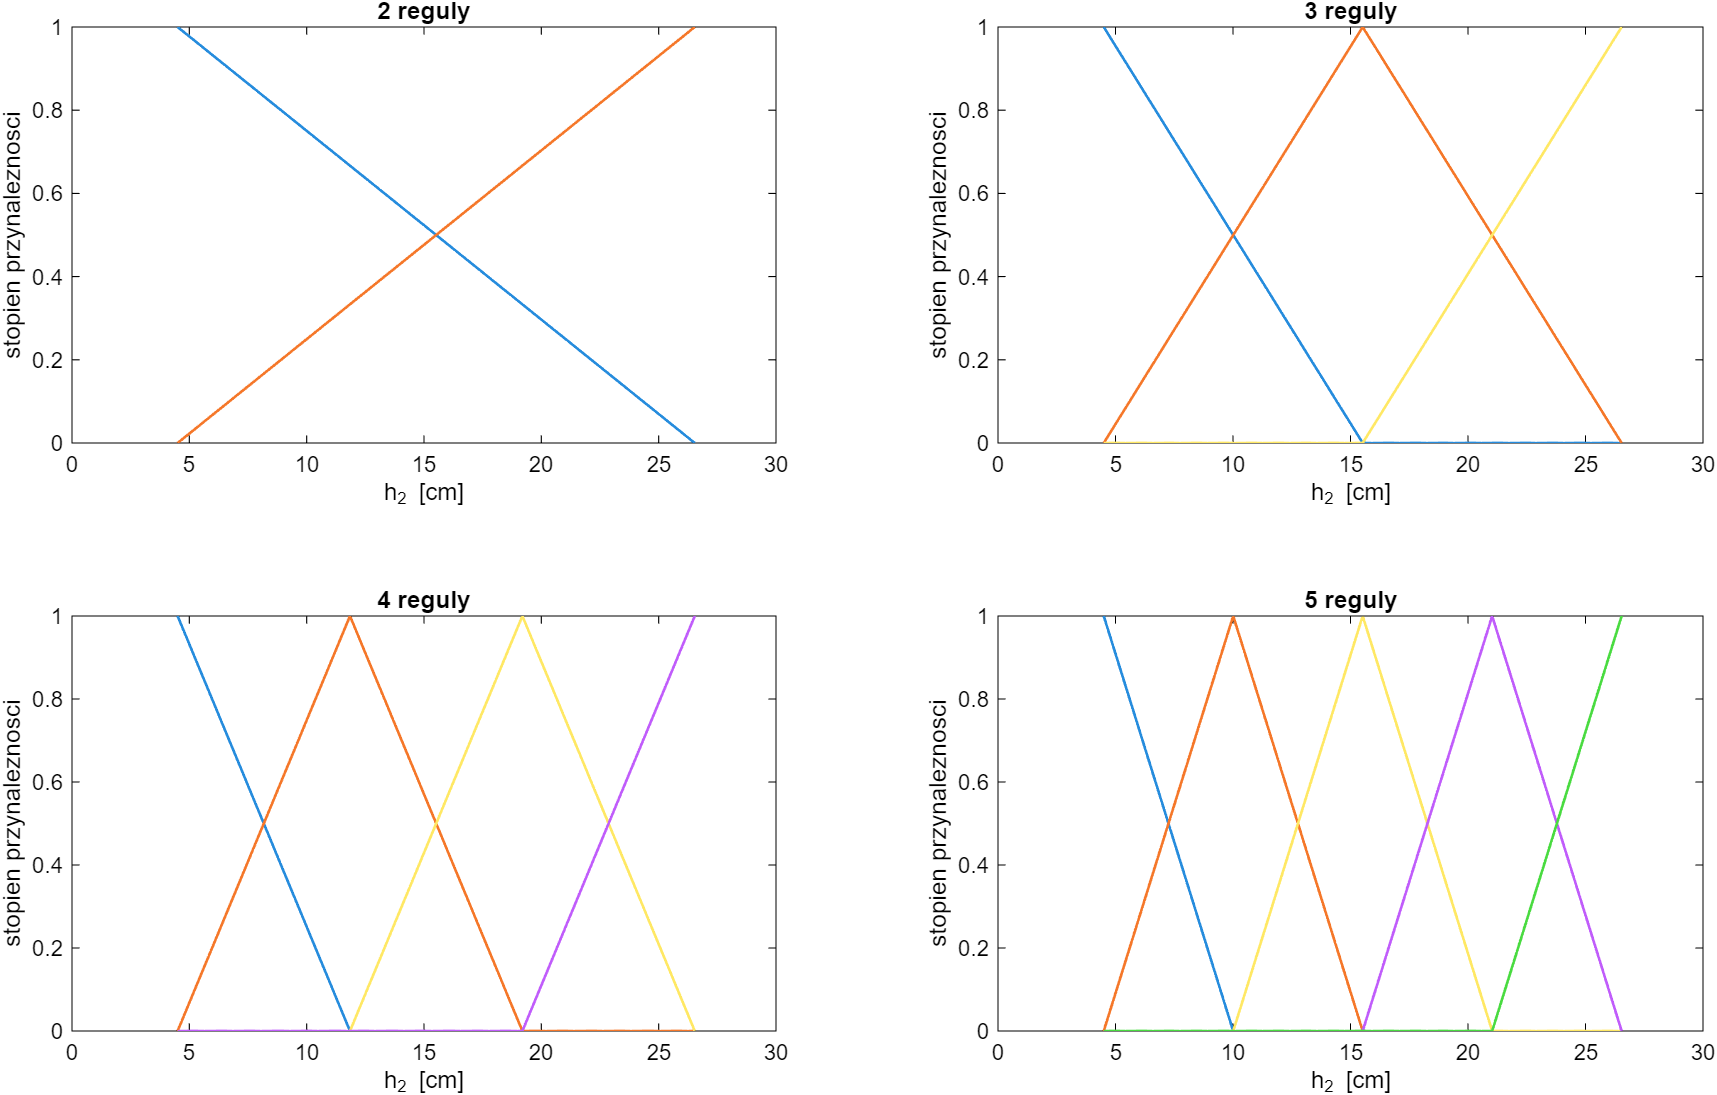
\includegraphics[width=0.92\textwidth]{rysunki/czesc2/funkcje_przynaleznosci.png}
\caption{Początkowe funkcje przynależności dla 2--5 reguł.}
\label{fig:ts-mf}
\end{figure}

\section{Porównanie jakości modeli}
Modele sprawdzono na 12 skokach z punktu pracy ($\Delta\uvar=\pm10,\pm25,\pm50\ \jednprzep$ oraz $\Delta F_D=\pm2,\pm5,\pm10\ \jednprzep$) w czasie $6000\ \mathrm{s}$. Błąd RMSE liczono względem obiektu nieliniowego po wszystkich próbkach; odniesieniem jest model liniowy z części~1.
\begin{table}[H]
\centering
\caption{Jakość modeli na 12 skokach z punktu pracy (przed strojeniem).}
\begin{tabular}{lrr}\toprule
Model & RMSE [cm] & Maksymalny błąd [cm]\\\midrule
Liniowy & \num{0.878} & \num{2.296}\\
TS, 2 reguły & \num{3.369} & \num{8.895}\\
TS, 3 reguły & \num{1.615} & \num{2.442}\\
TS, 4 reguły & \num{0.393} & \num{1.499}\\
TS, 5 reguł & \num{0.207} & \num{1.457}\\\bottomrule
\end{tabular}
\label{tab:ts-quality}
\end{table}

Dla 2 i 3 reguł uśrednianie szeroko rozstawionych linearyzacji przesuwa punkt równowagi modelu względem $h_{2,0}$ (widoczne już w pierwszych 200~s na rys.~\ref{fig:ts-models}). Od czterech reguł błąd spada poniżej modelu liniowego, a przy pięciu regułach RMSE osiąga \num{0.207}~cm -- ten model wybrano do dalszych badań. W tab.~\ref{tab:ts-amplitude} rozbito RMSE według amplitudy skoków obu wejść.

\begin{table}[H]
\centering
\caption{RMSE poziomu $h_2$ [cm] w zależności od amplitudy skoku.}
\small
\begin{tabular}{crrrrrr}\toprule
Amplituda & Liniowy & TS 2 & TS 3 & TS 4 & TS 5 & TS 5 strojony\\\midrule
10\% & \num{0.060} & \num{2.384} & \num{1.947} & \num{0.408} & \num{0.132} & \num{0.105}\\
25\% & \num{0.373} & \num{2.937} & \num{1.447} & \num{0.269} & \num{0.237} & \num{0.101}\\
50\% & \num{1.472} & \num{4.442} & \num{1.394} & \num{0.474} & \num{0.235} & \num{0.190}\\\bottomrule
\end{tabular}
\label{tab:ts-amplitude}
\end{table}

Dla małych skoków 10\% najdokładniejszy pozostaje model liniowy w punkcie pracy, natomiast przy zmianach 25\% i 50\% wyraźnie lepiej wypada model TS 5.

\begin{figure}[H]
\centering
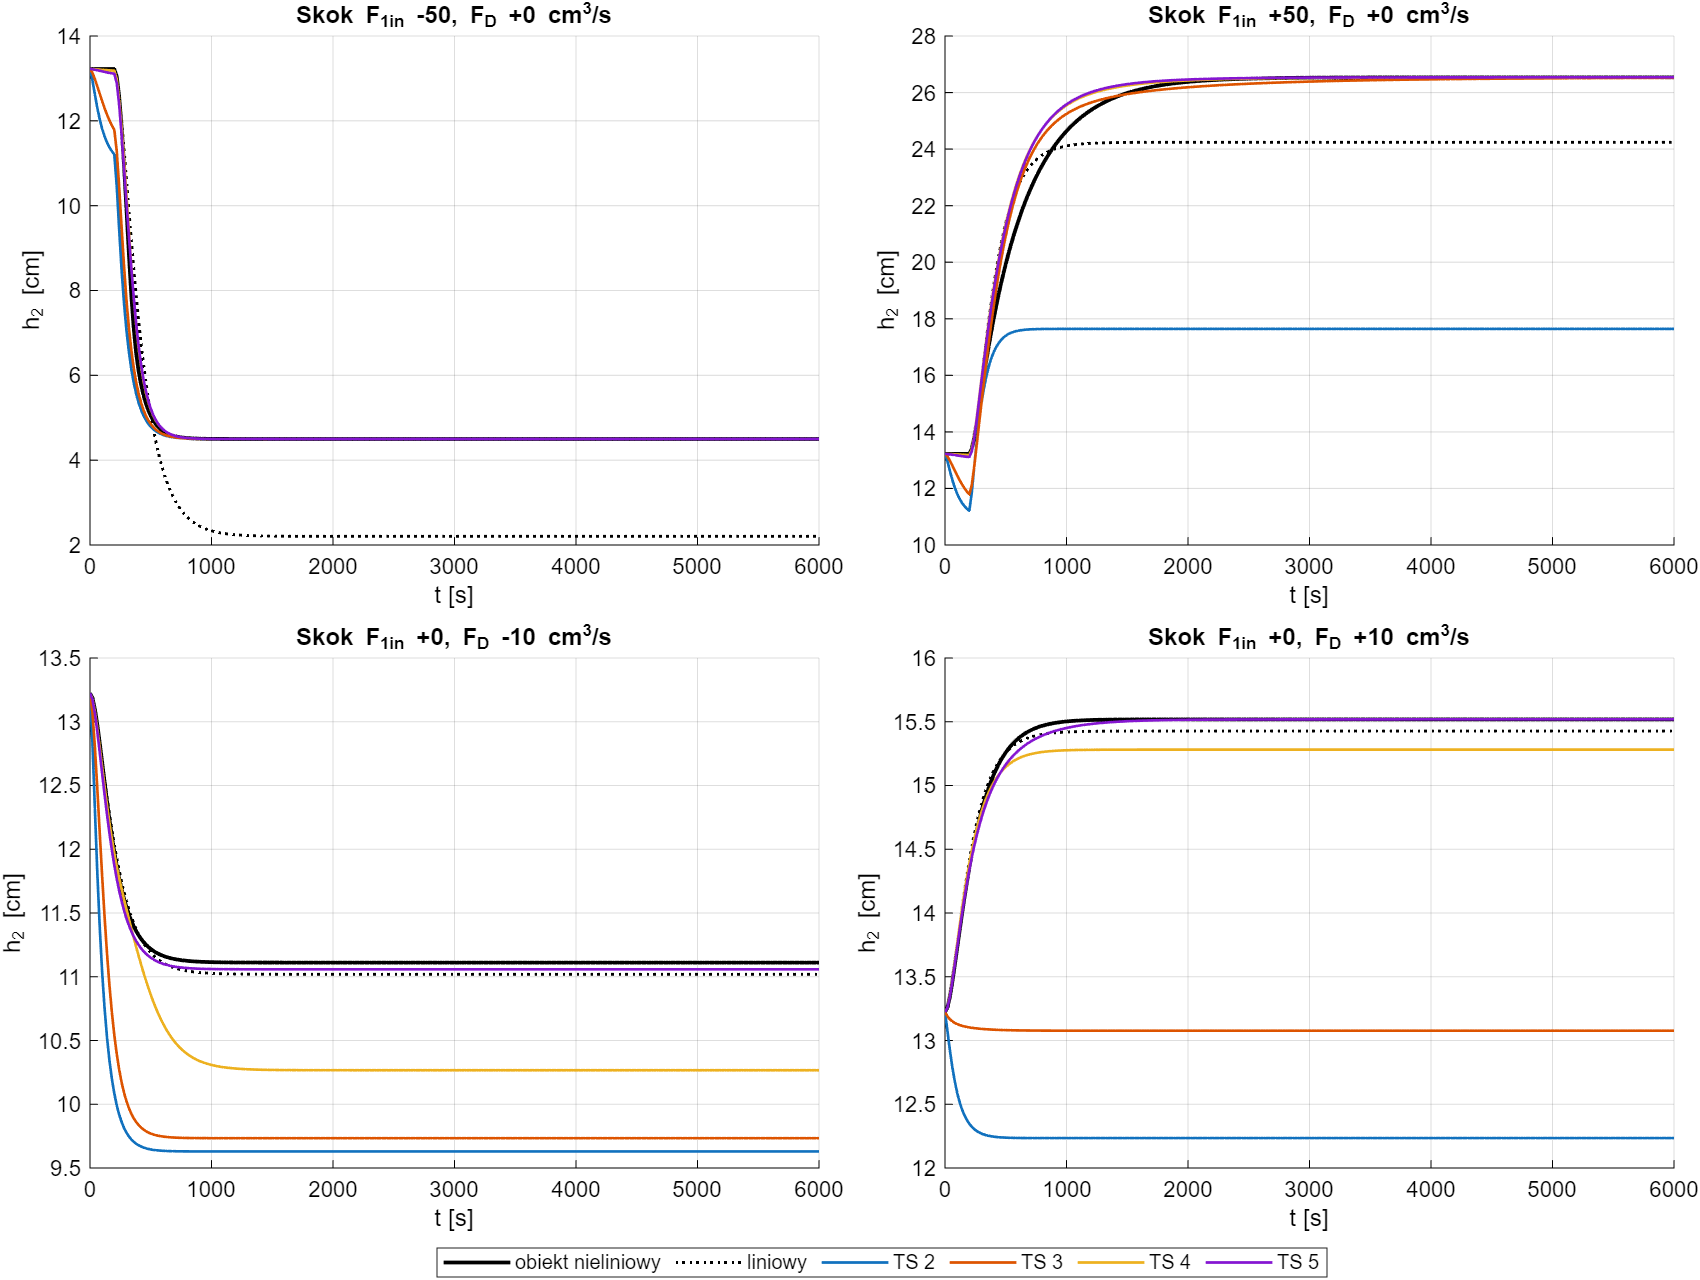
\includegraphics[width=\textwidth]{rysunki/czesc2/modele_2_5.png}
\caption{Odpowiedzi obiektu nieliniowego, modelu liniowego i modeli TS z 2--5 regułami.}
\label{fig:ts-models}
\end{figure}

\section{Strojenie funkcji przynależności modelu}
W modelu pięcioregułowym przesuwano trzy wewnętrzne węzły co 1~cm w zakresie $\pm2\ \mathrm{cm}$ przy stałych końcach przedziału i stałych następnikach. Węzły przed i po strojeniu wynoszą:
\begin{align*}
c_{\mathrm{przed}}&=[\num{4.500},\num{10.009},\num{15.519},\num{21.029},\num{26.538}]\ \mathrm{cm},\\
c_{\mathrm{po}}&=[\num{4.500},\num{8.009},\num{13.519},\num{19.029},\num{26.538}]\ \mathrm{cm}.
\end{align*}
Przesunięcie w stronę mniejszych poziomów poprawiło odwzorowanie w obszarze silniejszej nieliniowości. Łączny RMSE na 12 próbach spadł z \num{0.207} do \num{0.138}~cm (o \num{33.4}\%), a na 4 dodatkowych skokach walidacyjnych ($\Delta\uvar=\pm40$, $\Delta F_D=\pm7\ \jednprzep$) z \num{0.183} do \num{0.153}~cm.

\begin{figure}[H]
\centering
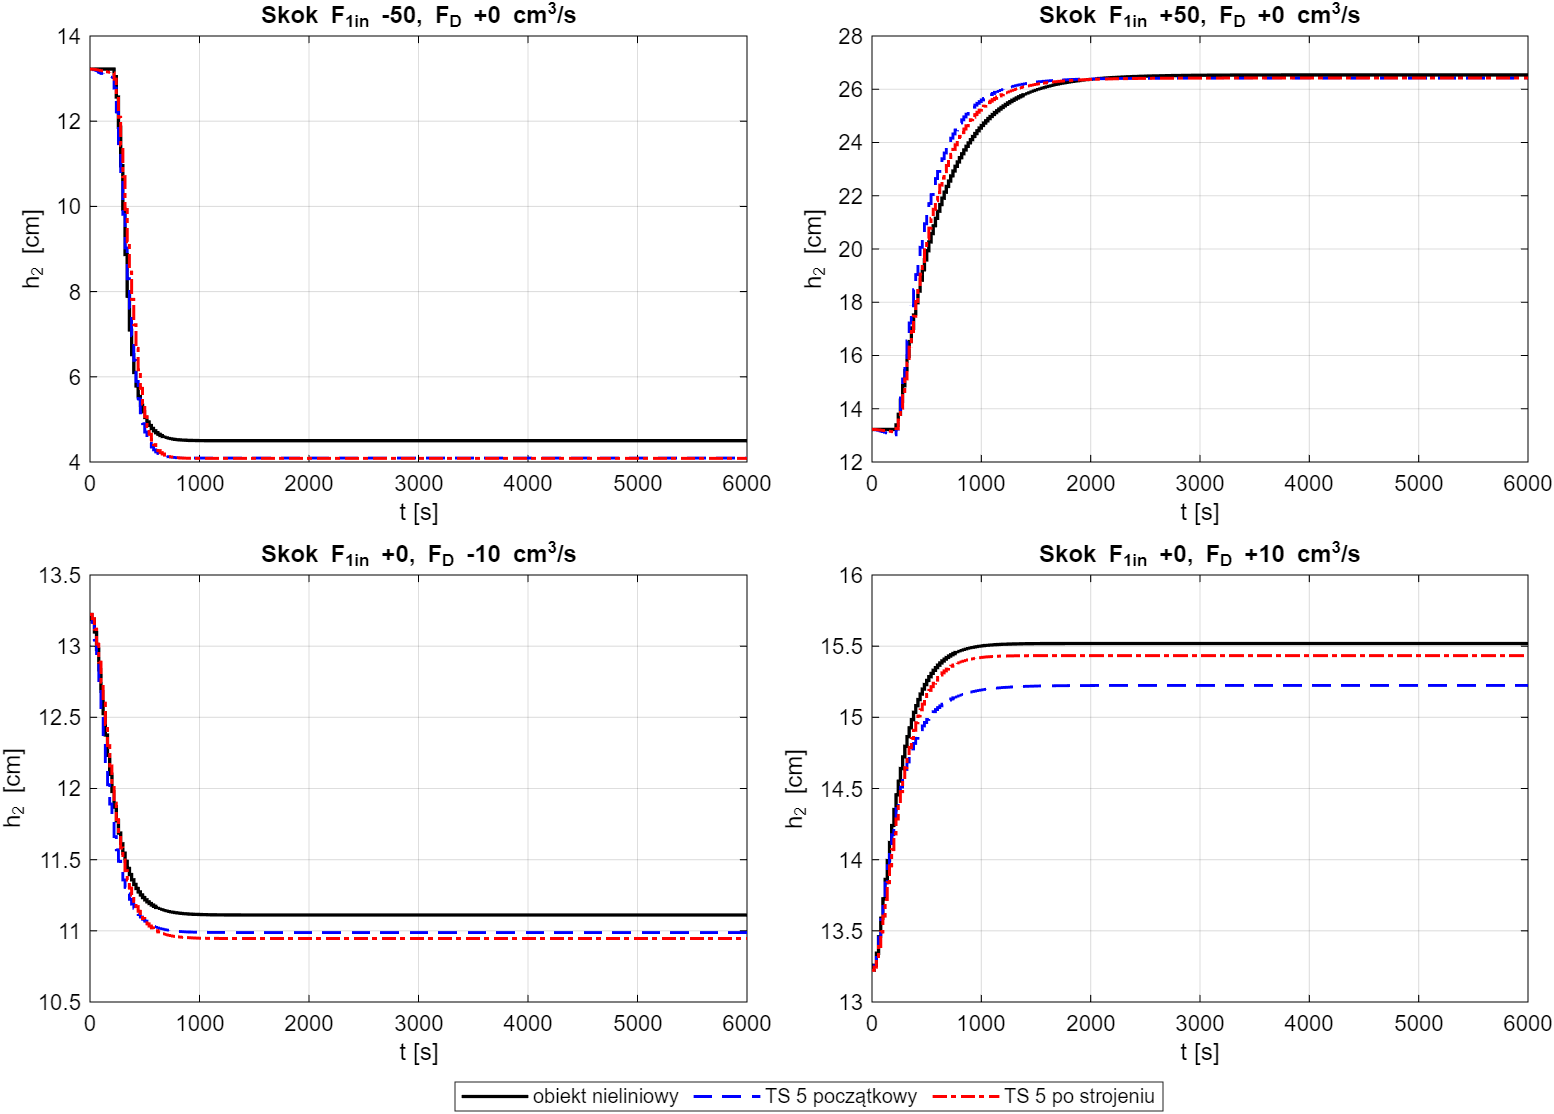
\includegraphics[width=0.95\textwidth]{rysunki/czesc2/porownanie_modeli_TS.png}
\caption{Model pięcioregułowy przed i po strojeniu funkcji przynależności.}
\label{fig:ts-tuned}
\end{figure}

\chapter{Analityczny rozmyty regulator predykcyjny (PDC)}
\section{Algorytm rozmytego DMC i ograniczenia}
Zgodnie z podejściem PDC (materiały wykładowe \emph{Regulatory rozmyte}, s.~148--149, wzory (4.72)--(4.75)) dla każdego z pięciu modeli lokalnych wyznaczono analityczny regulator DMC z odpowiedzi skokowej $s^{(i)}$. Zachowano nastawy z części~1: $D=250$, $N=50$, $N_u=10$, $\lambda=\num{0.05}$, $T_s=20\ \mathrm{s}$.

Dla $i$-tej reguły pierwszy wiersz $k_{1,i}^{\mathsf T}$ macierzy $K_i=(M_i^{\mathsf T}M_i+\lambda I)^{-1}M_i^{\mathsf T}$ wyznacza lokalny przyrost sterowania, a wypadkowy ruch rzutowany jest na ograniczenia:
\begin{align}
 Y_i^0(k)&=y(k)\mathbf 1+M_i^P\Delta U^P(k),\qquad
 \Delta u_i(k)=k_{1,i}^{\mathsf T}\bigl(Y_{\mathrm{zad}}(k)-Y_i^0(k)\bigr),\\
 \Delta u^*(k)&=\sum_{i=1}^5\widetilde w_i\bigl(y(k)\bigr)\,\Delta u_i(k),\\
 L(k)&=\max\bigl(-\Delta u_{\max},\,u_{\min}-u(k-1)\bigr),\qquad
 H(k)=\min\bigl(\Delta u_{\max},\,u_{\max}-u(k-1)\bigr),\\
 \Delta u(k)&=\min\bigl\{H(k),\,\max[L(k),\,\Delta u^*(k)]\bigr\}.
\end{align}
Przyjęto ograniczenia $0\leq\uvar\leq200\ \jednprzep$ i $|\Delta\uvar|\leq15\ \jednprzep$ na próbkę. Początkowe funkcje przynależności regulatora są takie same jak w dostrojonym modelu obiektu. Do porównania zestawiono nieograniczony DMC z części~1 oraz ten sam liniowy DMC z ograniczeniami.

\section{Porównanie układów i strojenie PDC}
Testy wykonano na tej samej osi czasu co w części~1: skok zadania w 400~s, skok $F_D$ w 3800~s, koniec w 8000~s. IAE liczono osobno dla zadania (400--3780~s) i zakłócenia (3800--8000~s).

Strojenie regulatora polegało na zmianie wyłącznie wag przełączania ($\widetilde w_i\propto\mu_i^\gamma$ dla $\gamma$ z zakresu od \num{0.5} do 3) i przesunięciu wewnętrznych węzłów o $\{-2,0,+2\}\ \mathrm{cm}$ przy stałych regulatorach lokalnych. Najmniejszy IAE dało $\gamma=\num{3.0}$ z węzłami $[\num{4.500},\num{10.009},\num{15.519},\num{21.029},\num{26.538}]\ \mathrm{cm}$ (rys.~\ref{fig:ts-controller-mf}).

\begin{figure}[H]
\centering
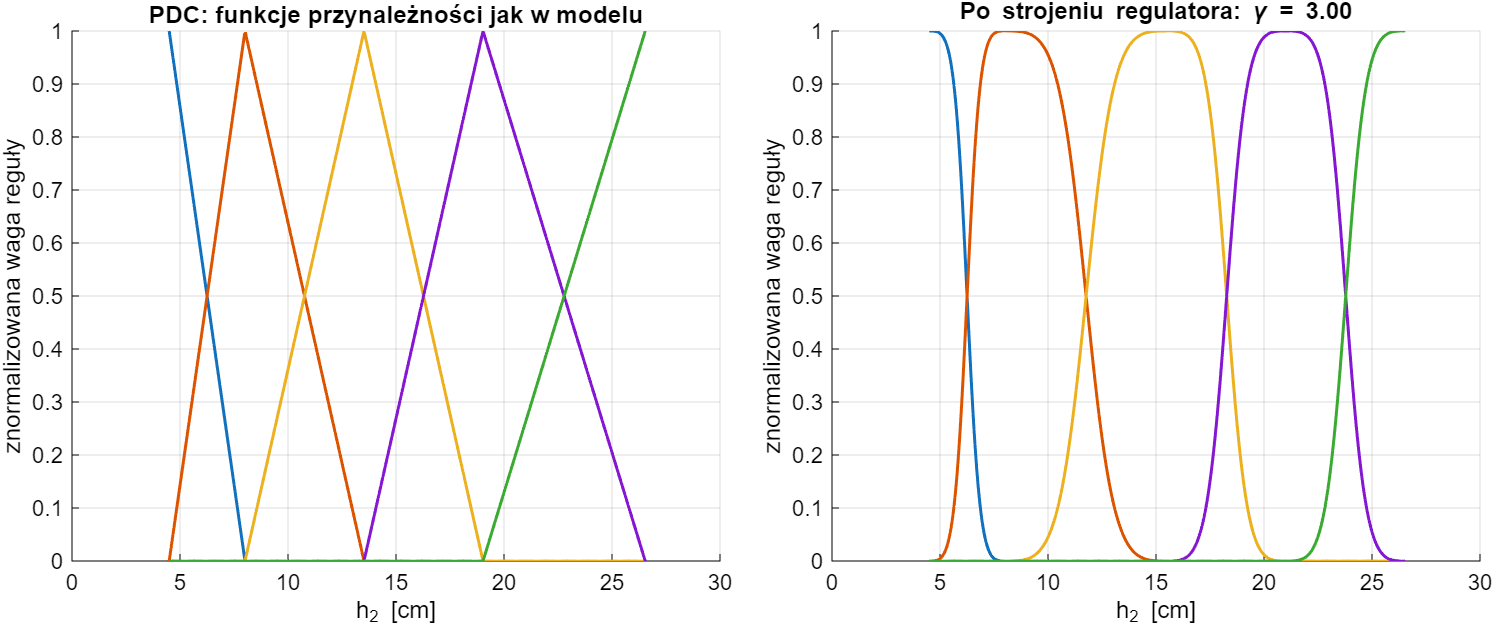
\includegraphics[width=0.94\textwidth]{rysunki/czesc2/strojenie_regulatora.png}
\caption{Funkcje przynależności regulatora PDC przed strojeniem ($\gamma=1$) i po strojeniu ($\gamma=3$).}
\label{fig:ts-controller-mf}
\end{figure}

\begin{table}[H]
\centering
\caption{Suma IAE zadania i zakłócenia w czterech próbach [cm$\cdot$s] ($N=50$, $N_u=10$, $\lambda=\num{0.05}$).}
\small
\begin{tabular}{lrrrr}\toprule
Skoki: zadanie / $F_D$ & DMC cz.~1 & Liniowy ogr. & PDC & PDC strojony\\\midrule
$+2\ \mathrm{cm}/+10\ \jednprzep$ & 1633 & 1633 & 1746 & 1573\\
$+4\ \mathrm{cm}/+20\ \jednprzep$ & 3944 & 3947 & 3809 & 3392\\
$+8\ \mathrm{cm}/+30\ \jednprzep$ & 9483 & 9627 & 7529 & 7001\\
$-8\ \mathrm{cm}/-10\ \jednprzep$ & 4443 & 4579 & 3187 & 3159\\\midrule
Suma & 19503 & 19785 & 16271 & 15125\\\bottomrule
\end{tabular}
\label{tab:ts-control}
\end{table}

Już początkowy PDC obniża sumę IAE o \num{17.8}\% względem ograniczonego DMC liniowego i wyraźnie ogranicza oscylacje przy skokach $\pm8\ \mathrm{cm}$ (rys.~\ref{fig:ts-control}). Po dostrojeniu wag łączny IAE spada o kolejne \num{7.0}\% (do 15\,125~cm$\cdot$s), poprawiając wynik DMC z części~1 o \num{22.5}\% w sumie i w każdej próbie osobno, mimo ograniczenia $|\Delta u|\leq15\ \jednprzep$ (DMC bez ograniczeń wykonywał ruchy do \num{31.12}~$\jednprzep$).

\begin{figure}[H]
\centering
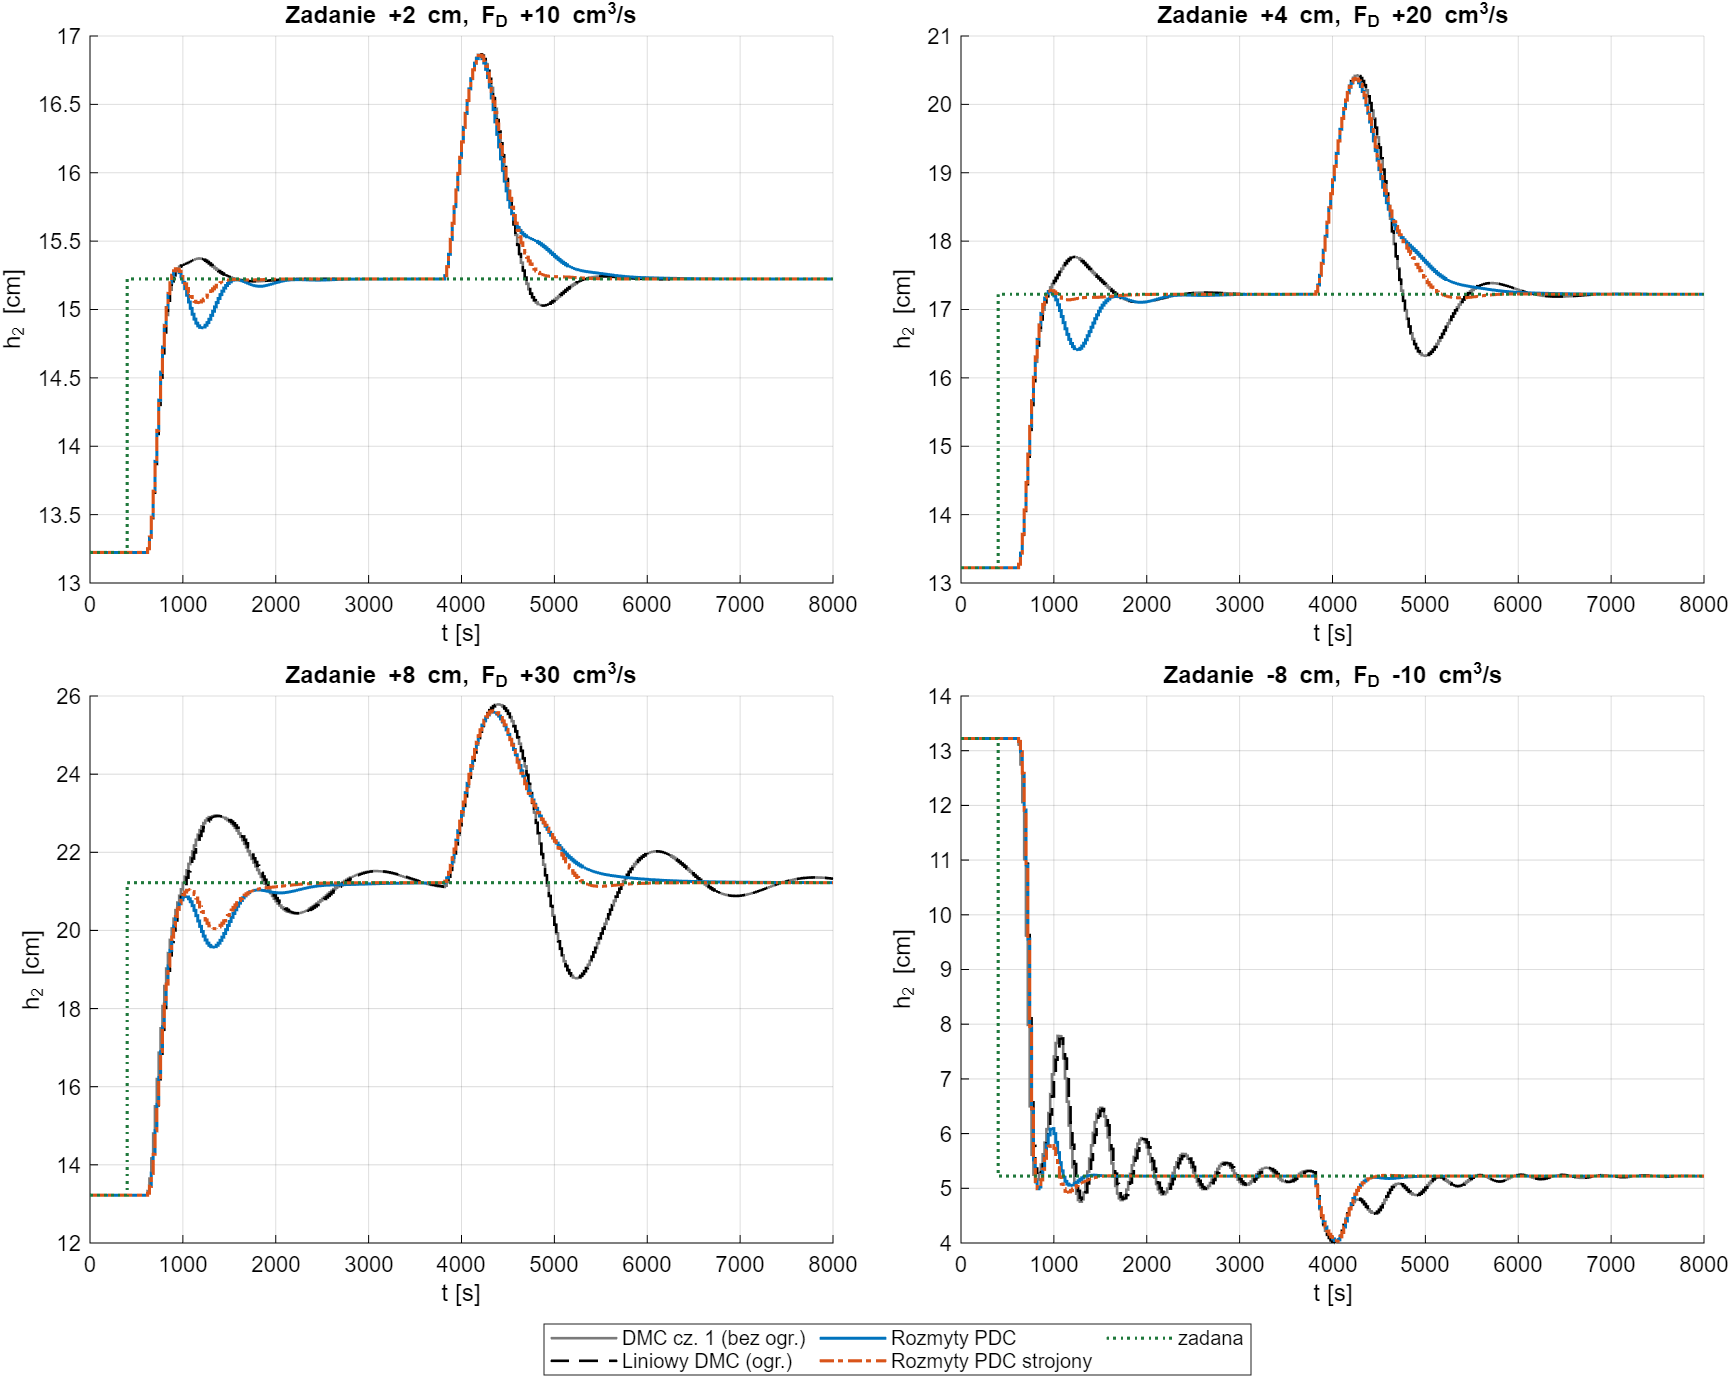
\includegraphics[width=\textwidth]{rysunki/czesc2/regulacja_porownanie.png}
\caption{Przebiegi poziomu $h_2$ dla DMC z części~1, ograniczonego DMC liniowego, PDC oraz PDC po strojeniu.}
\label{fig:ts-control}
\end{figure}
